\documentclass[runningheads]{llncs}

\usepackage[spanish]{babel}
\usepackage[T1]{fontenc}
\usepackage{graphicx}
\usepackage{wrapfig}
\usepackage{geometry}
\usepackage{hyperref}
\usepackage{url}
\usepackage{minted}
\usepackage{inconsolata}
\usepackage{caption}

\graphicspath{ {./img/} }
\geometry{
  a4paper,         % or letterpaper
  textwidth=15cm,  % llncs has 12.2cm
  textheight=24cm, % llncs has 19.3cm
  heightrounded,   % integer number of lines
  hratio=1:1,      % horizontally centered
  vratio=2:3,      % not vertically centered
}

\begin{document}

%
\title{Decompilación}
\titlerunning{Decompilación}

%
\author{
  Juan Bratti, 
  Emanuel Nicolás Herrador e
  Ignacio Scavuzzo
}
\authorrunning{J. Bratti, E. N. Herrador, I. Scavuzzo}

\institute{
  Facultad de Matemática, Astronomía, Física y Computación, Universidad Nacional de Córdoba, Argentina \\
  \email{juanbratti@mi.unc.edu.ar},
  \email{emanuel.nicolas.herrador@unc.edu.ar},
  \email{iscavuzzo@mi.unc.edu.ar}
}

\maketitle

%
\renewcommand{\abstractname}{Resumen}
\begin{abstract}
  El presente trabajo tiene como objetivo presentar un marco teórico sobre la decompilación de binarios.
  Se abordan las motivaciones detrás del desarrollo de los decompiladores junto con un breve contexto 
  histórico y los principales desafíos que conlleva esta tarea. Como referencia principal, se toma el 
  trabajo realizado por Cristina Cifuentes y John Gough, quienes hicieron un aporte significativo al 
  enfoque estático de la decompilación. En particular, describimos la arquitectura del decompilador 
  propuesto en su trabajo, \textit{dcc}, desarrollado para un procesador \textit{Intel 80286} y el 
  sistema operativo \textit{DOS}. Posteriormente, introducimos las técnicas de decompilación con enfoque 
  dinámico, señalando sus diferencias y ventajas frente al enfoque estático. Finalmente, se presentan 
  herramientas actuales y un caso de uso aplicando \textit{Ghidra} con el fin de ilustrar los conceptos 
  discutidos.
\end{abstract}

%
\section{Introducción}
En algunos ámbitos, como en el análisis de software y seguridad, se busca entender cómo funciona un 
programa partiendo únicamente de su binario. A veces, esta necesidad surge en contextos como la depuración,
la verificación o recuperación de software, donde se requiere entender qué hace un ejecutable sin necesidad 
de ejecutarlo ni tener conocimiento previo de su implementación.

La decompilación es la técnica que nos va a permitir transformar el binario de un programa en una 
representación legible, es decir, en un lenguaje de alto nivel. Sin embargo, esta técnica es compleja 
debido a varios desafíos como la pérdida de información durante la compilación y las técnicas de ofuscación 
o protección utilizadas para dificultar el uso de este tipo de herramientas.

Por estas razones, dentro del área se han explorado diversas implementaciones para abordar la decompilación, 
que van desde la recuperación precisa de la lógica que un programa tiene, hasta la generación de 
representaciones abstractas que se aproximen al programa original, a menudo dejando ciertas ambigüedades 
que requieren intervención o interpretación por parte del usuario.

Este informe tiene como objetivo presentar un marco teórico que permita entender los fundamentos de la 
decompilación, los distintos enfoques que se han llevado a cabo para implementar un decompilador, e 
introducir sus diversas aplicaciones. En principio, introduciremos la arquitectura de un decompilador 
tradicional estático, basándonos en el trabajo previo realizado por Cristina Cifuentes y John Gough.
Posteriormente, se hará una referencia a enfoques dinámicos, que buscan superar las limitaciones 
presentes en los enfoques estáticos. Finalmente, introduciremos algunos decompiladores modernos 
y sus aplicaciones.

%
\section{Contexto}
Un decompilador es un programa que pretende realizar el proceso inverso al de un compilador. 
Dado un ejecutable ya compilado, se desea obtener un programa de lenguaje de alto nivel que tenga 
la misma función \cite{cifuentes-dcc}.

Los primeros intentos de decompiladores surgieron en la década de $1960$ para su uso en la traducción 
de software para máquinas de nuevas generaciones. Estos lograban notar ambigüedades y código que no 
podían decompilar. En los $70$’ y $80$’, se usaban para modificar, documentar y debuggear binarios. 
Se utilizaban técnicas de \textit{pattern matching} de instrucciones de \textit{assembler}, o 
convenientemente, métodos con grafos. Posteriormente, surgieron aplicaciones en áreas como 
\textit{reverse engineering}, que pretenden obtener el código fuente a partir del objeto \cite{decompilation-methodology}.

Algunas aplicaciones de los decompiladores tienen como objetivo el entendimiento de librerías usadas 
por programadores o como paso intermedio para que el código sea recompilado con otro compilador \cite{meta-decompilation}, 
garantizando la correctitud sintáctica del código decompilado, la equivalencia semántica y la semejanza 
sintáctica con la fuente original. Además, son utilizados como prácticas de mantenimiento de software,
como migración de código a nuevas generaciones o traducción de código obsoleto a lenguajes estructurados \cite{cifuentes-dcc}.
Y, en cuanto a seguridad, para corregir fallas en ejecutables localizando los errores con decompilación \cite{decompilation-correctness}
y para el control de presencia de código malicioso \cite{cifuentes-dcc}.

En cuanto a los desafíos y problemas que surgen en su desarrollo, el principal es que la representación
de los datos y las instrucciones en arquitecturas de tipo Von Neumann es indistinguible: los datos pueden
estar entre instrucciones por ejemplo. También, destacamos que puede ocurrir que distintos programas
produzcan el mismo binario, o fragmentos iguales (debido a las optimizaciones hechas por el compilador).
Por otro lado, tenemos las subrutinas (como las provistas por librerías), que además de estar en el binario
que se quiere decompilar, suelen estar escritas en código assembler o en un binario y son difíciles de 
llevar a un \textit{high-level language} (HLL).  Por último, existen diversas cuestiones legales y morales
sobre la decompilación, principalmente en reverse engineering, ya que el software puede contener
código propietario (aunque generalmente se dificulta su decompilación con técnicas especiales de
ofuscación).

%
\section{Arquitectura de un Decompilador Tradicional}
En esta sección se presenta la arquitectura del decompilador estático \textit{dcc}. Esta herramienta
fue desarrollada para decompilar programas dirigidos al procesador \textit{Intel 80286} y al sistema
operativo \textit{DOS} \cite{cifuentes-dcc}. Su diseño se organiza en tres componentes o módulos principales, cada uno
con un rol específico dentro del proceso de decompilación.

\subsection{Front-end}
\begin{wrapfigure}{r}{0.3\textwidth}
  \vspace{-15pt}
  \centering
  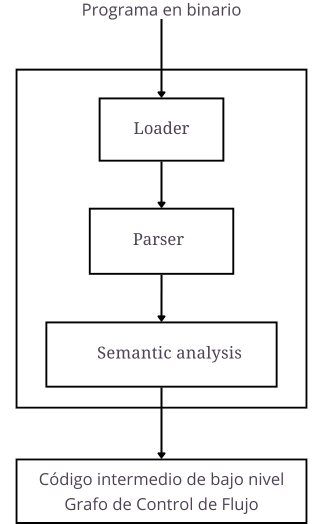
\includegraphics[width=0.3\textwidth]{frontend-phases.png}
  \caption{Fases del Front-end}
  \label{fig: frontend-phases}
  \vspace{-15pt}
\end{wrapfigure}

Este módulo será dependiente de la arquitectura del procesador, y es responsable de las tareas iniciales 
de desensamblado y análisis del binario. Tiene como principal objetivo convertir el código máquina en 
una representación intermedia de bajo nivel, preservando la semántica de las instrucciones originales.
Dentro del módulo tendremos varias etapas: la carga del binario en memoria virtual (\textit{loader}),
el desensamblado de instrucciones (\textit{parser}), el análisis semántico de instrucciones
(\textit{semantic analysis}), la creación de una representación intermedia del programa y la generación
del \textit{grafo de control de flujo} (\textit{CFG}). Estas etapas pueden verse gráficamente 
en la \autoref{fig: frontend-phases}.

Una vez se tiene el binario en memoria, el \textit{parser} comienza su trabajo convirtiendo las
instrucciones binarias en assembler. Esta conversión es secuencial y directa, excepto cuando se tienen
cambios en el control de flujo (saltos condicionales, llamados a procedimientos, por ejemplo). Cada vez
que se encuentra un cambio de flujo, se inicia una nueva ruta de desensamblado (es decir, se comienza
secuencialmente de nuevo, pero desde la parte del código a la que se saltó). 

Una vez desensambladas las rutas de ejecución, se procede a construir una representación intermedia
del código. Lo que se realiza es hacer una pseudo-instrucción por cada instrucción en assembler.
Por ejemplo, si se tiene la instrucción \verb|rep movs|, se mapea a la pseudo-instrucción
\verb|rep_movs|. Esta representación es luego usada para construir el grafo de control de flujo
que describe las relaciones entre los bloques del programa.

Luego, se lleva a cabo lo que se llama “semantic analysis”, en donde se busca reconocer 
\textit{idioms}\footnote{Un idiom es un patrón típico de instrucciones de bajo nivel que representa una 
operación semántica conocida.}. Estos \textit{idioms} se traducen a instrucciones intermedias más 
abstractas y legibles como puede verse en el ejemplo de la \autoref{fig: idioms-example}.

\begin{wrapfigure}{l}{0.33\textwidth}
  \centering
  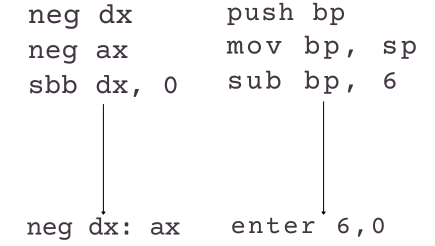
\includegraphics[width=0.33\textwidth]{idioms-example.png}
  \caption{Ejemplos de \textit{idioms} y sus transformaciones}
  \label{fig: idioms-example}
  \vspace{-15pt}
\end{wrapfigure}

Una vez identificados los \textit{idioms}, se aplica \textit{propagación de tipos} para identificar 
variables complejas como enteros largos o estructuras. Lo que se hace es deducir qué tipo de dato 
representa cada conjunto de accesos a memorias o registros para unificarlos como una sola variable 
de alto nivel. Por ejemplo, en una arquitectura de $16$ bits, si en assembler tenemos que se refiere 
a una variable de tipo \verb|long| ($32$ bits) de forma separada (debido a su largo se necesitan dos 
palabras de $16$ bits) lo que se hace es unificar ambas referencias en una sola, tratándola como 
una sola entidad lógica.

Finalmente, se lleva a cabo una optimización del grafo de control de flujo donde se busca 
simplificar el flujo eliminando redundancias y acortando saltos.

\subsection{Máquina de Decompilación Universal (UDM)}
\begin{wrapfigure}{r}{0.35\textwidth}
  \vspace{-15pt}
  \centering
  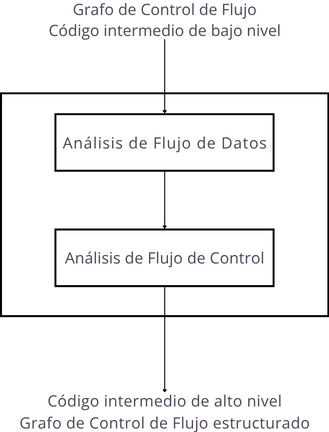
\includegraphics[width=0.35\textwidth]{udm-phases.png}
  \caption{Fases de la UDM}
  \label{fig: udm-phases}
  \vspace{-20pt}
\end{wrapfigure}

Este módulo constituye el núcleo del decompilador, y se va a encargar de transformar la
representación intermedia de bajo nivel generada por el \textit{front-end} en una forma más abstracta
y estructurada (para acercarnos al lenguaje de alto nivel deseado). Su funcionamiento se divide en
$2$ subfases: \textit{análisis de flujo de datos} y \textit{análisis de flujo de control}, las cuales 
pueden visualizarse en la \autoref{fig: udm-phases}.

Es importante destacar que este módulo se abstrae de la arquitectura del procesador y del lenguaje 
objetivo de alto nivel (de allí la palabra “Universal” en su nombre), pudiendo usar este módulo
independientemente de la arquitectura del procesador y del lenguaje objetivo de alto nivel.

\paragraph{Análisis de flujo de datos} En esta subfase se busca transformar las representaciones 
de bajo nivel obtenidas, en una representación de alto nivel (HLL), es decir, en un lenguaje 
fácil de leer y entender por un humano. Para ello, se eliminan conceptos que no existen en 
lenguajes HLL (por ejemplo registros y flags) y se introducen expresiones algebraicas.

Para las instrucciones que utilizan \textit{flags}, se intenta traducir aquellas que sí tienen 
una expresión de alto nivel equivalente (esto depende del tipo de flag que la instrucción este utilizando).
En caso de tratarse de una flag que puede ser traducida a alto nivel, se realiza un análisis de uso 
y definición (\textit{use/definition chain}) para identificar la instrucción que definió la flag y 
la que usó la flag. Esta identificación permite luego traducir ambas instrucciones en una instrucción de 
alto nivel semánticamente equivalente como puede verse en el ejemplo de la \autoref{fig: flags-delete}.

\begin{wrapfigure}{l}{0.5\textwidth}
  \vspace{-15pt}
  \centering
  
\includegraphics[width=0.5\textwidth]{flags-delete.png}
  \caption{Ejemplo de código con flags}
  \label{fig: flags-delete}
  \vspace{-15pt}
\end{wrapfigure}

La semántica de la instrucción \verb|JCOND| de la \autoref{fig: flags-delete} es equivalente a realizar 
\verb|cmp+jg| en una sola expresión, sin necesidad de utilizar de manera explícita las flags. 
Esto es porque \verb|jg| usa las flags que \verb|cmp| setea al ejecutarse.

Para las instrucciones que utilizan registros, lo que se hace es reemplazar instrucciones de bajo 
nivel que usan registros intermedios o temporales, por instrucciones de alto nivel que no (de nuevo,
esto depende del tipo de instrucción). Para aquellas instrucciones que si pueden reemplazarse por 
instrucciones de alto nivel, lo que se hace es también hacer un análisis de uso y definición 
(\textit{use/definition chain}) para reemplazar secuencias de instrucciones que definen y usan un 
registro temporal por una sola instrucción que semánticamente haga lo mismo. 
Por ejemplo, si se tiene que un registro temporal contiene el resultado de \verb|5+bx| y se 
usa inmediatamente después, se elimina el registro y se expresa directamente la operación.

\begin{figure}[!htb]
  \centering
  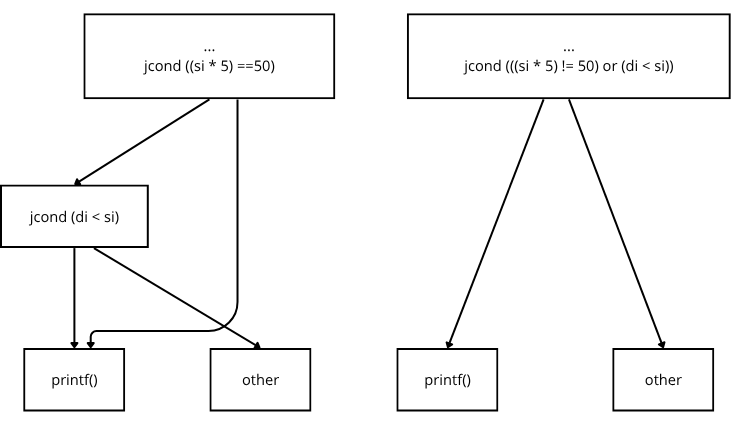
\includegraphics[width=0.7\textwidth]{optimized-cfg.png}
  \caption{Grafos optimizados y reestructurados}
  \label{fig: optimized-cfg}
  \vspace{-15pt}
\end{figure}

\paragraph{Análisis de flujo de control} En esta otra subfase se reestructura el CFG del programa para 
transformarlo en estructuras de control genéricas de alto nivel como \verb|if … then[… else]|, 
\verb|while()| o \verb|repeat…until()|, etc. Para hacer esto se utiliza un algoritmo para detectar 
en el CFG subgrafos que se puedan mapear a esas estructuras. Si algún subgrafo no tiene mapeo, 
utiliza goto como último recurso.

Luego de hacer esta reestructuración, se optimizan los grafos para tener condiciones compuestas 
como \verb+if(a || b)+ en lugar de hacer uso de \verb|if| anidados (\autoref{fig: optimized-cfg}).

\subsection{Back-end}
Finalmente, este último módulo pretende generar el código en un lenguaje de alto nivel. 
Este módulo depende del lenguaje que se quiera generar, ya que tiene que adaptar las representaciones 
obtenidas por el UDM a construcciones sintácticas específicas del lenguaje. Podemos diferenciar 
el trabajo de este módulo en dos subfases: \textit{reestructuración} (opcional) y 
\textit{generación de código} (\autoref{fig: backend-phases}).

\begin{wrapfigure}{r}{0.35\textwidth}
  \vspace{-25pt}
  \centering
  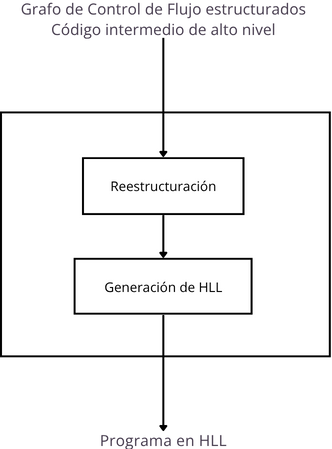
\includegraphics[width=0.35\textwidth]{backend-phases.png}
  \caption{Fases del Back-end}
  \label{fig: backend-phases}
  \vspace{-50pt}
\end{wrapfigure}

\paragraph{Reestructuración} Esta subfase es opcional y en ella se reestructura el grafo devuelto por 
la UDM, adaptándolo a las construcciones que el lenguaje destino pueda tener. La razón de que sea 
opcional es porque sólo mejora la calidad del código generado.

\paragraph{Generación de código} En esta subfase se procede a generar el código para el grafo de 
control devuelto por la UDM (o por la etapa de \textit{Reestructuración}) y las instrucciones 
intermedias de alto nivel (también devuelto por la UDM). Se definen las variables globales y se 
genera el código para cada función o procedimiento. Los nombres de las variables y 
funciones/procedimientos son arbitrarios y genéricos, al igual que las etiquetas para los goto.
Al generar el código, también se genera documentación adicional en forma de comentarios, 
en donde se incluye detalles como el uso de registros para argumentos de funciones, qué registros 
se usaron como retorno de funciones, entre otros.

\section{Limitaciones del Enfoque Estático}
La implementación del decompilador mostrado se basa en decompilación estática, en donde se analiza 
el binario de un programa y se reconstruye su sintaxis en un lenguaje de alto nivel sin ejecutar el 
binario, solamente a partir de construcciones intermedias como los CFG y los lenguajes HLL.

Sin embargo, este enfoque estático presenta varias desventajas \cite{binrec}. Algunas de ellas son:

\paragraph{Problemática 1. Código vs Datos y ambigüedad de referencias} El código máquina no diferencia 
explícitamente entre lo que son datos e instrucciones, ambos comparten el mismo espacio de memoria 
pero no son lo mismo. Por ello, algunos bytes podrían ser interpretados como instrucciones inválidas 
cuando en realidad representan datos.

\paragraph{Problemática 2. Control de Flujo Indirecto} Los enfoques estáticos no son muy buenos 
manejando saltos indirectos (saltos que no van a una dirección fija si no a donde diga un registro 
o la memoria), y algunas veces las heurísticas no son suficientes para reconstruir con exactitud 
un salto en este tipo condiciones, haciendo que se pierda la semántica original de un programa.

\paragraph{Problemática 3. Omisión de Datos Externos} En general, los programas pueden hacer uso de
funciones o valores externos proveniente de librerías, y si bien existen algunas implementaciones 
en el enfoque estático que buscan remediar esta limitación\footnote{Por ejemplo, el decompilador dcc 
implementa dccSign para tratar llamadas a librerías}, en general sólo se centran únicamente en el código 
máquina del programa original, sin tener un contexto adecuado para poder entender o reconstruir el 
programa completo de forma correcta.

\paragraph{Problemática 4. Código ofuscado} Existen programas que están diseñados de tal manera que 
no es fácil analizar o detectar qué hacen. En estos casos, se emplean técnicas que cambian el flujo 
lógico o hacen parecer que el mismo está desordenado, llevando la complejidad del programa a tal 
punto que los decompiladores estáticos son incapaces de reconstruir correctamente su semántica.\newline

Es por estas desventajas que se han tomado otros enfoques a la hora de realizar decompilación. 
A continuación introducimos uno de ellos.

\section{Enfoque Dinámico en la Decompilación}
En base a las limitaciones encontradas para los decompiladores estáticos, se plantearon diferentes 
enfoques de decompilación más avanzados como \textit{dynamic binary lifting} (como se implementa 
en la librería Binrec\footnote{Librería open source que funciona muy bien para binarios en la 
práctica, pasando muchos de los benchmarks para frameworks de este tipo. 
Disponible en: \url{https://github.com/trailofbits/binrec-tob}.}) \cite{binrec}. A diferencia de 
los métodos estáticos, las herramientas de DBT (\textit{dynamic binary translation}) analizan ejecuciones 
de un programa, manejando componentes como código y datos mezclados. Binrec transforma código 
a una versión intermedia de alto nivel llamada LLVM IR, que actúa como abstracción, para 
luego transformarlo y bajarlo de nuevo a binario.

La herramienta permite analizar código que una herramienta estática no puede. Sin embargo, 
surge un problema. Cuando se levanta el programa se observa una traza específica de ejecución, 
pero no todas las posibles. Binrec lo soluciona implementando handlers, que eventualmente pueden 
aplicar \textit{incremental lifting}, lo que permite refinar el binario según se descubra nuevo código.

\section{Herramientas Actuales y Caso de Estudio}
Durante la última década, la investigación y el desarrollo de decompiladores y de análisis de binarios 
avanzó notablemente. Un hito clave para ello fue la publicación de Ghidra por parte de 
la Dirección en Investigación de la NSA (National Security Agency) el 4 de abril de 2019 \cite{ghidra-book},
haciendo posible un análisis profundo y detallado de binarios sin necesidad de requerir herramientas 
comerciales de alto costo como \textit{IDA Pro}.

Actualmente, existen múltiples decompiladores especializados para distintas arquitecturas y distintos 
lenguajes tanto intermedios como de alto nivel. Así mismo, existen herramientas dedicadas al análisis 
de binarios que se enfocan en el análisis simbólico utilizando la representación intermedia y sin 
necesidad de requerir una decompilación en un lenguaje de alto nivel. Estas herramientas, como 
\textit{angr}, pueden utilizarse para realizar tareas como detección de malware, análisis de control 
de flujo y detección de vulnerabilidades.

Las herramientas de decompilación y análisis de binarios más relevantes en la actualidad son 
Ghidra\footnote{Plataforma open source desarrollada por la NSA que incluye un desensamblador, 
un decompilador a C y herramientas de análisis estático sobre múltiples arquitecturas. Disponible 
en \url{https://github.com/NationalSecurityAgency/ghidra}.}, IDA Pro\footnote{Herramienta 
comercial de análisis binario que combina desensamblado interactivo con análisis avanzado y 
opcionalmente el decompilador Hex-Rays para obtener pseudocódigo en C. Más información 
en \url{https://hex-rays.com/ida-pro}.}, \textit{RetDec}\footnote{Decompilador modular open source 
desarrollado por Avast que convierte binarios en pseudocódigo en C. Disponible 
en \url{https://github.com/avast/retdec}.}, \textit{Binary Ninja}\footnote{Plataforma de análisis 
binario comercial (con versión gratuita limitada) que utiliza múltiples representaciones intermedias, 
incluye su propio decompilador y soporta scripting y automatización. Más información 
en \url{https://binary.ninja/}.} (y su plugin \textit{dewolf}\footnote{Plugin experimental open 
source de Binary Ninja para decompilación, diseñado con fines académicos para producir pseudocódigo 
más legible, enfocado en el análisis manual. Disponible en \url{https://github.com/fkie-cad/dewolf}.}), 
\textit{angr}\footnote{Framework en Python (librería) open source para análisis binario automatizado, 
que utiliza representación intermedia a VEX y permite ejecución simbólica y análisis de rutas.
Disponible en \url{https://github.com/angr/angr}.} y \textit{radare2}\footnote{Conjunto de herramientas 
open source para análisis forense e ingeniería inversa a bajo nivel, con soporte para desensamblado,
depuración, scripting y modificación de binarios. Disponible en: 
\url{https://github.com/radareorg/radare2}.}. En el presente trabajo, nos centraremos en 
Ghidra para nuestro caso de estudio, aplicado a un programa simple.

El programa considerado implementa Fibonacci en C++ (\autoref{apendice:fibonacci} del apéndice) y el binario correspondiente contiene 
la información de depuración\footnote{Se obtiene compilando sin optimización y con la flag \texttt{-g}.}
para mejorar la legibilidad de los resultados de la decompilación. Usando la plataforma de Ghidra,
se obtienen dos funciones principales a tener en cuenta, \verb|main| (\autoref{apendice:main-decompilation-with-depuration-info} del apéndice) y \verb|swap<>| (\autoref{apendice:swap-decompilation-with-depuration-info} del apéndice).
En ambas funciones se puede observar que al principio de su cuerpo se realiza la declaración de una variable 
aleatoria (\verb|local_10| y \verb|lVar1|) y al final se corrobora que ese valor se haya mantenido. 
Este es un ejemplo de funcionalidades agregadas por el compilador a nuestro código fuente debido a que 
es un chequeo de seguridad automático para protección contra \textit{stack smashing} (para evitar 
ataques para sobrescribir valores de la pila y cambiar direcciones de retorno, modificar el comportamiento 
del programa y demás).

Otro aspecto a mencionar en la función \verb|main| es la claridad a la hora de mostrar el manejo 
de input y de output mediante la utilización de variables de tipo \verb|istream| y \verb|otream|, y
los operadores \verb|>>| y \verb|<<|. Además, se reconoce el bucle \verb|for| (en caso de no tener 
información de depuración, el loop hubiera sido reconocido pero colocado como un \verb|while|) y la 
llamada a la función \verb|swap|. Notar que las funciones y variables mantienen su nombre porque es 
información que se dejó al compilar con información de depuración.

Finalmente, en cuanto a la función \verb|swap|, puede observarse que es una función donde los parámetros 
se pasan por referencia (en particular, Ghidra muestra que se pasan los punteros a lo valores)
y se hace el swap de estos con tres instrucciones de asignación.

Gracias a este caso de uso simple, puede notarse el potencial e importancia de los decompiladores 
al poder reconstruir un programa con una semántica equivalente al programa original e incluso buscando 
equivalencia sintáctica en algunas partes si se dispone de la información (es decir, no es información 
que se desecha durante la compilación u optimizaciones en la misma). Usualmente Ghidra
y las demás herramientas se utilizan para el análisis de binarios más sofisticados y grandes, que 
requieren un análisis exhaustivo y preciso para, por ejemplo, la identificación de vulnerabilidades.

\section{Conclusión}
Como hemos visto, la decompilación representa una herramienta clave en el análisis de software,
ya sea con fines de depuración, recuperación o de seguridad. Este informe abordó sus fundamentos teóricos,
los principales desafíos técnicos y la arquitectura modular del decompilador estático dcc. 
Además, se introdujo el enfoque dinámico para contrastar las limitaciones de los decompiladores 
estáticos, y se exploraron herramientas de decompilación como Ghidra a través de ejemplos concretos 
para poder ilustrar los resultados de un decompilador moderno. 

Pudimos observar, gracias al trabajo realizado, el potencial que los decompiladores y las herramientas 
de análisis binarios tienen para poder inspeccionar archivos ejecutables, identificar estructuras 
y analizar el comportamiento del código original. Sin embargo, estas herramientas aún presentan 
limitaciones como la identificación correcta de los tipos de datos o la semejanza sintáctica sin 
dependencia de la información de depuración, por lo que este sector continúa siendo un área de 
investigación en constante desarrollo, crucial para la ingeniería inversa y con un gran impacto 
en la seguridad informática y otros campos. Actualmente, con el desarrollo e implementación de 
los modelos de inteligencia artificial, se está avanzando a decompiladores con enfoques híbridos 
que utilizan estos modelos para mejorar la legibilidad y comprensión del código de alto nivel generado.

\bibliographystyle{splncs04}
\bibliography{references}

\section*{Apéndice}

\begin{minipage}{0.95\linewidth}
\begin{minted}[linenos]{c}
#include <iostream>

int main() {
  std::cout << "Enter two natural values: ";
  std::cout.flush();

  long long n, m;
  std::cin >> n >> m;

  std::cout << "Fibonacci sequence (first " << n << " values modulo " << m
            << "):\n";
  long long bef = 0, aft = 1;
  for (int i = 0; i < n; i++) {
    std::cout << "\tfib[" << i << "] = " << bef << '\n';
    std::swap(bef, aft);
    aft = (aft + bef) % m;
  }

  return 0;
}
\end{minted}
\captionof{figure}{Implementación de Fibonacci en C++}
\label{apendice:fibonacci}
\end{minipage}

\begin{minipage}{0.95\linewidth}
\begin{minted}[linenos]{c}
int main(void)
{
  istream *this;
  ostream *poVar1;
  long in_FS_OFFSET;
  int i;
  longlong n;
  longlong m;
  longlong bef;
  longlong aft;
  long local_10;
  
  local_10 = *(long *)(in_FS_OFFSET + 0x28);
  std::operator<<((ostream *)std::cout,"Enter two natural values: ");
  std::ostream::flush();
  this = (istream *)std::istream::operator>>((istream *)std::cin,&n);
  std::istream::operator>>(this,&m);
  poVar1 = std::operator<<((ostream *)std::cout,"Fibonacci sequence (first ");
  poVar1 = (ostream *)std::ostream::operator<<(poVar1,n);
  poVar1 = std::operator<<(poVar1," values modulo ");
  poVar1 = (ostream *)std::ostream::operator<<(poVar1,m);
  std::operator<<(poVar1,"):\n");
  bef = 0;
  aft = 1;
  for (i = 0; i < n; i = i + 1) {
    poVar1 = std::operator<<((ostream *)std::cout,"\tfib[");
    poVar1 = (ostream *)std::ostream::operator<<(poVar1,i);
    poVar1 = std::operator<<(poVar1,"] = ");
    poVar1 = (ostream *)std::ostream::operator<<(poVar1,bef);
    std::operator<<(poVar1,'\n');
    std::swap<>(&bef,&aft);
    aft = (bef + aft) % m;
  }
  if (local_10 != *(long *)(in_FS_OFFSET + 0x28)) {
                    /* WARNING: Subroutine does not return */
    __stack_chk_fail();
  }
  return 0;
}
\end{minted}
\captionof{figure}{Decompilación propuesta por Ghidra para \texttt{main} de Fibonacci con información de depuración}
\label{apendice:main-decompilation-with-depuration-info}
\end{minipage}

\begin{minipage}{0.95\linewidth}
\begin{minted}[linenos]{c}
void std::swap<>(longlong *__a,longlong *__b)
{
  long lVar1;
  longlong lVar2;
  long in_FS_OFFSET;
  longlong *__b_local;
  longlong *__a_local;
  longlong __tmp;
  
  lVar1 = *(long *)(in_FS_OFFSET + 0x28);
  lVar2 = *__a;
  *__a = *__b;
  *__b = lVar2;
  if (lVar1 != *(long *)(in_FS_OFFSET + 0x28)) {
                    /* WARNING: Subroutine does not return */
    __stack_chk_fail();
  }
  return;
}
\end{minted}
\captionof{figure}{Decompilación propuesta por Ghidra para \texttt{swap} de Fibonacci con información de depuración}
\label{apendice:swap-decompilation-with-depuration-info}
\end{minipage}

\end{document}
